%%%%%%%%%%%%%%%%%%%%%%%%%%%%%%%%%%%%%%%%%%%%%%%%%%%%%%%%%%%%%%%%%%%%%%%%%%%
%
% Generic template for TFC/TFM/TFG/Tesis
%
% $Id: introduccion.tex,v 1.19 2015/02/24 23:21:54 macias Exp $
%
% By:
%  + Javier Macías-Guarasa. 
%    Departamento de Electrónica
%    Universidad de Alcalá
%  + Roberto Barra-Chicote. 
%    Departamento de Ingeniería Electrónica
%    Universidad Politécnica de Madrid   
% 
% Based on original sources by Roberto Barra, Manuel Ocaña, Jesús Nuevo,
% Pedro Revenga, Fernando Herránz and Noelia Hernández. Thanks a lot to
% all of them, and to the many anonymous contributors found (thanks to
% google) that provided help in setting all this up.
%
% See also the additionalContributors.txt file to check the name of
% additional contributors to this work.
%
% If you think you can add pieces of relevant/useful examples,
% improvements, please contact us at (macias@depeca.uah.es)
%
% Copyleft 2013
%
%%%%%%%%%%%%%%%%%%%%%%%%%%%%%%%%%%%%%%%%%%%%%%%%%%%%%%%%%%%%%%%%%%%%%%%%%%%

\chapter{Background}\label{chp:background}

%%%%%%%%%%%%%%%%%%%%%%%%%%%%%%%%%%%%%%%%%%%%%%%%%%%%%%%%%%%%%%%%%%%%%%%%%%%%%%%%
\section{Data Complexity Metrics}\label{sec:ecol}

There are many complexity metrics that could be used for the scope of this 
project, but it has been chosen the ones that are explained below; following 
the metrics obtained from~\cite{BasuH2006}, and surveys by Lorena et 
al~\cite{lorena2018,Lorena2019}. They are also implemented in the Extended 
Complexity Metrics Library (ECoL) for R.

These are a set of measures that help characterizing the complexity of 
classification and regression problems. The measures that are going to be 
computed for this project are:

\begin{description}
    \item [Overlapping] Evaluate how informative the available features are to 
    separate the classes. See \ref{sec:overlap} for more details.
    \item [Neighborhood] Characterize the presence and density of classes in 
    local neighborhoods. See \ref{sec:neighborhood} for more details.
    \item [Linearity] Quantify, if it is possible, whether classes are linear 
    separable by a hyperplane or linear function. See \ref{sec:linearity} for 
    more details.
    \item [Dimensionality] Indicative of data sparsity, how smoothly samples are
    distributed within attributes. See \ref{sec:dimesionality} for more details.
    \item [Balance] Capture the difference in the number of examples per class 
    in the dataset. See \ref{sec:balance} for more details.
    \item [Network] Represents the dataset as a graph and extracts structural 
    information out of it. See \ref{sec:network} for more details.
    \item [Correlation] Relationship between the feature values and the outputs.
    See \ref{sec:correlation} for more details. 
    \item [Smoothness] In regression problems, the smoother the function to be
    fitted to the data, the simpler it shall be. See \ref{sec:smoothness} for 
    more details.
\end{description}

These complexity measures are going to be computed for certain datasets and
comparisons between results are going to be made.

%%%%%%%%%%%%%%%%%%%%%%%%%%%%%%%%%%%%%%%%%%%%%%%%%%%%%%%%%%%%%%%%%%%%%%
\subsection{Measures of Overlap of Individual Feature Values}\label{sec:overlap}

An overlapped dataset is defined as a multi-class dataset where the data is 
interlaced. The meaning of this statement is explained as follows: having a 
dataset whose geometrical expression have the domain, $D_n$\footnote{Being 
\textit{n} the number of attributes for that class}, a second class will have a 
domain, $D'_n$, intersecting that of the first class.

%%%%%%%%%%%%%%%%%%%%%%%%%%%%%%%%%%%%%%%%%%%%%%%%%%%%%%%%%%%%
\subsubsection{Fisher's Discriminant Ratio (F1)}\label{sec:f1}

This metric is specific to one feature dimension. Even if the given problem is 
multidimensional, not necessarily all features have to contribute to class 
discrimination, only one of the features needs to be the discriminant. 
Fulfilling this statement would ease the complexity of the problem.

The measure uses the following mathematical expression:

\[ f = \frac{(\mu _1 - \mu _2)^2}{\sigma _1^2 + \sigma _2^2} \]

Where \(\mu _1,\mu _2,\sigma _1^2, \sigma _2^2\) are the means and variances, 
respectively, of the two classes\footnote{It has been used two classes for the 
definition of the metric, but more classes could be added to the problem.}.

%%%%%%%%%%%%%%%%%%%%%%%%%%%%%%%%%%%%%%%%%%%%%%%%%%%%%%%%%%%%
\subsubsection{Directional Vector Fishers Discriminant Ratio (F1v)}

Complemented F1 (see Section~\ref{sec:f1}). It does so by searching for a vector
capable of separating two classes after the training  samples have been projected
into it.

%%%%%%%%%%%%%%%%%%%%%%%%%%%%%%%%%%%%%%%%%%%%%%%%%%%%%%%%%%%%
\subsubsection{Volume of Overlap Region (F2)}

Another way to measure the complexity is by using the tails of the overlap of 
the classes. This is accomplished by taking the maximum and minimum values of 
each class. Afterwards, the length of overlap is calculated, normalized by 
range of the classes. This is done by:

\[ f = \prod_{i} \frac{MIN(max(f_i, c_1), max(f_i, c_2)) - MAX(min(f_i, c_1), min(f_i, c_2))}{MAX(max(f_i, c_1), max(f_i, c_2)) - MIN(min(f_i, c_1), min(f_i, c_2))}\]

Where \(f_i\) indicates the feature; \(c_n\) indicates the class; and \(i\) 
indicates the dimensionality of the problem.

%%%%%%%%%%%%%%%%%%%%%%%%%%%%%%%%%%%%%%%%%%%%%%%%%%%%%%%%%%%%
\subsubsection{Feature Efficiency (F3)}\label{sec:f3}

In this measure, in high-dimensional problems, each feature is evaluated 
separately on how much it contributes to the separation of the classes. If 
there exists overlap within the range of each class for a certain feature, the 
class is considered to be ambiguous for that dimension in the specific region 
where the overlap takes place.

Therefore a problem will be more feasible if the exists at least one feature 
where the ranges for each class do not overlap. Thus, the \textit{maximum 
feature efficiency} will be used as a measure. This measure is obtained with 
the entire training set, by obtaining the remaining points being separable by 
the feature.

%%%%%%%%%%%%%%%%%%%%%%%%%%%%%%%%%%%%%%%%%%%%%%%%%%%%%%%%%%%%
\subsubsection{Collective Feature Efficiency (F4)}

It gives an overview on how different features may work together in data 
separation. The most discriminant feature (see F3 - \ref{sec:f3}) is selected 
and then all samples separable by this feature are removed from the dataset.
This process is repeated with all the features until no samples are left.
The resulting value of this metric comes from the ratio of samples that
have been discriminated.

%%%%%%%%%%%%%%%%%%%%%%%%%%%%%%%%%%%%%%%%%%%%%%%%%%%%%%%%%%%%%%%%%%%%%%
\subsection{Measures of Neighborhood}\label{sec:neighborhood}

For a certain set of target classes in a dataset, the neighborhood measures
try to analyze the neighbor data items of every data point and try to capture
class overlapping and the shape of the decision boundary. The work is done
over a distance matrix which stores distances between all pairs of data points
in the dataset.

%%%%%%%%%%%%%%%%%%%%%%%%%%%%%%%%%%%%%%%%%%%%%%%%%%%%%%%%%%%%
\subsubsection{Mixture Identifiability (N1, N2, N3)}

The measure is defined as the mean Euclidean distance from each point in the 
dataset, to its nearest neighbors, not minding the class they are in
\cite{FriedmanRafsky}. The valuable rates that can be taken are the means 
for interclass neighbors and intraclass neighbors.

%%%%%%%%%%%%%%%%%%%%%%%%%%%%%%%%%%%%%%%%%%%%%%%%%%%%%%%%%%%%
\subsubsection{Non-linearity of the Nearest Neighbor Classifier (N4)}

It builds a new dataset by interpolating pairs of training samples of the same  
class and the induce a 1NN classifier on the original data and measure the error
rate in the new data points.

%%%%%%%%%%%%%%%%%%%%%%%%%%%%%%%%%%%%%%%%%%%%%%%%%%%%%%%%%%%%
\subsubsection{Fraction of Hyper-spheres Covering Data (T1)}

It creates a hyper-sphere centered at each one of the training samples. Their
radios are then growth until one hyper-sphere reaches a sample of other class.
Then, smaller hyper-spheres contained in larger hyper-spheres are eliminated.
This measure is the ratio between the number of remaining hyper-spheres and the
total number of samples in the dataset. 

%%%%%%%%%%%%%%%%%%%%%%%%%%%%%%%%%%%%%%%%%%%%%%%%%%%%%%%%%%%%
\subsubsection{Local Set Average Cardinality (LSC)}

It is a set of points from the dataset whose distance of each sample is smaller
than the distance from the samples of the different classes. 

%%%%%%%%%%%%%%%%%%%%%%%%%%%%%%%%%%%%%%%%%%%%%%%%%%%%%%%%%%%%%%%%%%%%%%
\subsection{Measures of Separability of Classes}\label{sec:linearity}

Given two, or more classes, inside a certain dataset, they can be called linear 
separable if a straight line between those classes can be drawn. As the 
previous statement suggests, the classes must be isolated clusters after the 
linear function is delimited.

%%%%%%%%%%%%%%%%%%%%%%%%%%%%%%%%%%%%%%%%%%%%%%%%%%%%%%%%%%%%
\subsubsection{Linear Separability (L1, L2, L3)}

As a way to adapt to separable and non-separable problems, it is used the 
formulation proposed by Smith\cite{FWSmith}, which minimizes an error function:

\begin{align*} 
 \text{minimize } a^{t}t \\
 \text{subject to } Z^{t}w + t \geq b \\
 t \geq 0 
\end{align*}

Implying that a and b are vectors; w is the weight vector; t is the error 
vector and Z is a matrix obtained by adding one dimension, with value one, to 
the input vector x.

%%%%%%%%%%%%%%%%%%%%%%%%%%%%%%%%%%%%%%%%%%%%%%%%%%%%%%%%%%%%%%%%%%%%%%
\subsection{Measures of Dimensionality}\label{sec:dimesionality}

For any dataset, the dimensionality measures will indicate data sparsity.
These measures capture how sparse a dataset tends to have regions of low 
density. These regions have been proven to be harder for the extraction of 
good classification and regression models.

%%%%%%%%%%%%%%%%%%%%%%%%%%%%%%%%%%%%%%%%%%%%%%%%%%%%%%%%%%%%
\subsubsection{Average Number of samples per dimension (T2)}

It represents the average number of points per dimension. It is calculated with 
the ratio between the number of examples and dimensionality of the dataset.

%%%%%%%%%%%%%%%%%%%%%%%%%%%%%%%%%%%%%%%%%%%%%%%%%%%%%%%%%%%%
\subsubsection{Average intrinsic dimensionality per number of samples (T3)}

Another way to measure the dimensionality of a dataset, is by computing the 
average of number of points per PCA. It is a similar measure to $T2$, which
uses the number of PCA components needed to represent 95 variability as
the base of a data sparsity assessment.

%%%%%%%%%%%%%%%%%%%%%%%%%%%%%%%%%%%%%%%%%%%%%%%%%%%%%%%%%%%%
\subsubsection{Intrinsic dimensionality proportion (T4)}

It represents a ratio of PCA Dimensions to the Original. It returns an estimate 
of the proportion of relevant and original dimensions of the dataset.

%%%%%%%%%%%%%%%%%%%%%%%%%%%%%%%%%%%%%%%%%%%%%%%%%%%%%%%%%%%%%%%%%%%%%%
\subsection{Measures of Class Balance}\label{sec:balance}

Given a certain dataset, \textit{balance} measures capture the differences in
the number of samples per class for that dataset. When the imbalance ratio is 
too severe, problems related to generalization of classification techniques 
could happen.

%%%%%%%%%%%%%%%%%%%%%%%%%%%%%%%%%%%%%%%%%%%%%%%%%%%%%%%%%%%%
\subsubsection{Entropy of class proportions (C1)}

This measure captures the imbalance of a dataset using proportions of 
samples per class.

%%%%%%%%%%%%%%%%%%%%%%%%%%%%%%%%%%%%%%%%%%%%%%%%%%%%%%%%%%%%
\subsubsection{Multi-class imbalance ratio (C2)}

The ratio at hand represents an index calculated to measure a class balance.
It is not only suited for binary class classification problems, but also is  
suited for multi-class classification problems.

%%%%%%%%%%%%%%%%%%%%%%%%%%%%%%%%%%%%%%%%%%%%%%%%%%%%%%%%%%%%%%%%%%%%%%
\subsection{Measures of Network}\label{sec:network}

These measures create a graph representation of the dataset to extract 
structural information from it. The transformation between raw data and the
graph representation is based on the epsilon-NN ($\varepsilon-NN$) algorithm.
Afterwards, a post-processing step is applied to the graph, pruning edges
between samples of opposite classes.

%%%%%%%%%%%%%%%%%%%%%%%%%%%%%%%%%%%%%%%%%%%%%%%%%%%%%%%%%%%%
\subsubsection{Average density of of network (Density)}

It is a representation of the count of edges in the graph, divided by the 
maximum number of edges between pairs of data points.

%%%%%%%%%%%%%%%%%%%%%%%%%%%%%%%%%%%%%%%%%%%%%%%%%%%%%%%%%%%%
\subsubsection{Clustering Coefficient (ClsCoef)}

Computes the average of the clustering tendency of the vertices by the ratio
of existent edges between neighbors and the total number of edges that could
possibly exist between them.

%%%%%%%%%%%%%%%%%%%%%%%%%%%%%%%%%%%%%%%%%%%%%%%%%%%%%%%%%%%%
\subsubsection{Average hub score (Hubs)}

Is given by the number of connections to other nodes, weighted by the amount
of connections the neighbors have.

%%%%%%%%%%%%%%%%%%%%%%%%%%%%%%%%%%%%%%%%%%%%%%%%%%%%%%%%%%%%%%%%%%%%%%
\subsection{Measures of Feature Correlation}\label{sec:correlation}

A regression task that calculate the correlation of the values of the features
to the outputs. In case one feature is highly correlated to the output, it is
understandable that simpler functions can be fitted to the data.

%%%%%%%%%%%%%%%%%%%%%%%%%%%%%%%%%%%%%%%%%%%%%%%%%%%%%%%%%%%%
\subsubsection{Maximum/Average feature correlation to the output (C1, C2)}

Representation of the maximum/average value of the Spearman correlations for 
each feature and the output.

%%%%%%%%%%%%%%%%%%%%%%%%%%%%%%%%%%%%%%%%%%%%%%%%%%%%%%%%%%%%
\subsubsection{Individual feature efficiency (C3)}

Returns the number of samples to be removed from the dataset to reach a high 
Spearman correlation value to the output.

%%%%%%%%%%%%%%%%%%%%%%%%%%%%%%%%%%%%%%%%%%%%%%%%%%%%%%%%%%%%
\subsubsection{Collective feature efficiency (C4)}

Gives the ratio of samples removed from the dataset based on an iterative 
process of linear fitting between the features and the target attribute.

%%%%%%%%%%%%%%%%%%%%%%%%%%%%%%%%%%%%%%%%%%%%%%%%%%%%%%%%%%%%%%%%%%%%%%
\subsection{Measures of Smoothness}\label{sec:smoothness}

It is a regression task, used for regression problems. In those problems, the 
smoother the function to be fitted, the simpler the task it becomes. Large 
variations in input/output are an indication of the existence of more intricate
relationships between them.

%%%%%%%%%%%%%%%%%%%%%%%%%%%%%%%%%%%%%%%%%%%%%%%%%%%%%%%%%%%%
\subsubsection{Output distribution (S1)}

Checks if the samples joined in then MST have similar output values. The lower
the value, the simpler the problem - where outputs of similar samples in the 
input space are also next to each other.

%%%%%%%%%%%%%%%%%%%%%%%%%%%%%%%%%%%%%%%%%%%%%%%%%%%%%%%%%%%%
\subsubsection{Input distribution (S2)}

Monitors the similarity in the input space of data items with similar outputs
based on distance.

%%%%%%%%%%%%%%%%%%%%%%%%%%%%%%%%%%%%%%%%%%%%%%%%%%%%%%%%%%%%
\subsubsection{Error of a nearest neighbor regressor (S3)}

Stands for the mean squared error of a 1-nearest neighbor regressor using 
leave-one-out.

%%%%%%%%%%%%%%%%%%%%%%%%%%%%%%%%%%%%%%%%%%%%%%%%%%%%%%%%%%%%
\subsubsection{Non-linearity of nearest neighbor regressor (S4)}

Computes the mean squared error of a 1-nearest neighbor regressor to the new 
randomly interpolated points.

\begin{center}
\begin{scriptsize}
\begin{longtable}{ | r | l | l | c | c | c | }
\caption{Complexity Metrics from \cite{Lorena2019} and 
\cite{Lorena2017}}\label{tab:all-metrics} \\

\hline
\textit{\textbf{Category}}        &
\textit{\textbf{Name}}            &
\textit{\textbf{Acronym}}         &
\textit{\textbf{Min}}             &
\textit{\textbf{Max}}             &
\textit{\textbf{Asymptotic Cost}} \\
\hline
\hline
\endfirsthead
\hline
\multicolumn{6}{c}{\tablename\ \thetable\ -- \textit{Continued from previous page}} \\
\hline \\
\endhead
\hline
\textit{\textbf{Category}}        &
\textit{\textbf{Name}}            &
\textit{\textbf{Acronym}}         &
\textit{\textbf{Min}}             &
\textit{\textbf{Max}}             &
\textit{\textbf{Asymptotic Cost}} \\
\hline
\hline
\endfoot
\hline
\endlastfoot

\multirow{5}{*}{Feature-based} & Maximum Fisher's discriminant ratio & 
F1 & $\approx0$ & 1 & $O(m \cdot n)$ \\ 
\cline{2-6}
& Directional vector maximum Fisher's discriminant ratio &
F1v & $\approx0$ & 1 & $O(m \cdot n \cdot n_{c} + m^3 \cdot n^2_c)$ \\
\cline{2-6}
& Volume of overlapping region &
F2 & 0 & 1 & $O(m \cdot n \cdot n_{c})$ \\ 
\cline{2-6}
& Maximum individual feature efficiency &
F3 & 0 & 1 & $O(m \cdot n \cdot n_{c})$ \\ 
\cline{2-6}
& Collective feature efficiency &
F4 & 0 & 1 & $O(m^{2} \cdot n \cdot n_{c})$ \\ 
\hline

\multirow{6}{*}{Neighborhood} & Faction of borderline points &
N1 & 0 & 1 & $O(m \cdot n^2)$ \\ 
\cline{2-6}
& Ratio of intra/extra class NN distance &
N2 & 0 & $\approx 1$ & $O(m \cdot n^2)$ \\
\cline{2-6}
& Error rate of NN classifier &
N3 & 0 & 1 & $O(m \cdot n^2)$ \\
\cline{2-6}
& Non linearity of NN classifier &
N4 & 0 & 1 & $O(m \cdot n^2 + m \cdot l \cdot n)$ \\ 
\cline{2-6}
& Fraction of hyper-spheres covering data &
T1 & 0 & 1 & $O(m \cdot n^2)$ \\
\cline{2-6}
& Local set average cardinality &
LSC & 0 & $1 - \frac{1}{n}$ & $O(m \cdot n^2)$ \\
\hline

\multirow{3}{*}{Linearity} & Sum of the error distance by linear programming & 
L1 & 0 & $\approx 1$ & $O(n^2)$ \\ 
\cline{2-6}
& Error rate of linear classifier &
L2 & 0 & 1 & $O(n^2)$ \\ 
\cline{2-6}
& Non linearity of linear classifier &
L3 & 0 & 1 & $O(n^{2} + m \cdot n \cdot n_{c})$ \\ 
\cline{2-6}
\hline

\multirow{3}{*}{Dimensionality} & Average number of features per dimension &
T2 & $\approx 0$ & $m$ & $O(m + n)$ \\ 
\cline{2-6}
& Average number of PCA dimensions per points & 
T3 & $\approx 0$ & $m$ & $O(m^2 \cdot n + m^3)$ \\
\cline{2-6}
& Ratio of the PCA dimension to the original dimension &
T4 & 0 & 1 & $O(m^2 \cdot n + m^3)$ \\
\hline

\multirow{2}{*}{Class Imbalance} & Entropy of classes proportions &
C1 & 0 & 1 & $O(n)$ \\
\cline{2-6}
& Imbalance ratio &
C2 & 0 & 1 & $O(n)$ \\
\hline

\multirow{3}{*}{Network} & Density &
Density & 0 & 1 & $O(m \cdot n^2)$ \\
\cline{2-6}
& Clustering Coefficient &
ClsCoef & 0 & 1 & $O(m \cdot n^2)$ \\
\cline{2-6}
& Hubs & 
Hubs & 0 & 1 & $O(m \cdot n^2)$ \\
\hline

\multirow{4}{*}{Correlation} & Maximum Feature Correlation to the Output &
C1 & 0 & 1 & $O(n \cdot m \cdot log m)$ \\
\cline{2-6}
& Average Feature Correlation to the Output &
C2 & 0 & 1 & $O(n \cdot m \cdot log m)$ \\
\cline{2-6}
& Individual Feature Efficiency &
C3 & 0 & 1 & $O(n \cdot m^2)$ \\
\cline{2-6}
& Collective Feature Efficiency &
C4 & 0 & 1 & $O(n \cdot (d + n \cdot log n))$ \\
\hline

\multirow{3}{*}{Smoothness} & Output Distribution & 
S1 & 0 & - & $O(n^2)$ \\
\cline{2-6}
& Input Distribution &
S2 & 0 & - & $O(m \cdot (n + log m))$ \\
\cline{2-6}
& Error of a nearest neighbor regressor &
S3 & 0 & - & $O(n^2)$ \\
\hline

\end{longtable}
\end{scriptsize}
\end{center}

%%%%%%%%%%%%%%%%%%%%%%%%%%%%%%%%%%%%%%%%%%%%%%%%%%%%%%%%%%%%%%%%%%%%%%%%%%%%%%%%
\section{Supervised Classification}

Machine Learning has different methods or styles available:

\begin{description}
    \item [Supervised] Trains itself on labeled data set.
    \item [Unsupervised] Ingests unlabeled data and uses algorithms to extract 
    meaningful features needed to label or sort data - without human
    intervention.
    \item [Semi-supervised] Uses smaller labeled dataset to set up a guide and 
    large amounts of unlabeled data for feature extraction
\end{description}

In this work, the only the first of them is used. Getting into more detail on
supervised learning, it means that the machine learning model is built on
data that has enough labeled information on how to determine and classify new
incoming data.

That could be the example of a model ready to identify dogs. Many images with 
dogs, that would label the breed, and other characteristics, would be necessary 
to differentiate an Alaskan Malamute from a Beagle.

Now, it is true that this technique requires less input data to train a model,
which make it easier to obtain a decent amount of data to train and test the
model. Also, data can easily be tested, thanks to labeled data - which is a bit
more expensive to generate than unlabelled data (for obvious reasons). There is
also the danger of overfitting the model. It means that the model is too close
to the training set. It is translated to a poor performance over slight 
variations from new data.

In supervised learning, an optimal scenario is considered when the model is able
to label correctly unseen data (which might come from a testing set or from new
data).

Other applications, that have not been mentioned so far, could be database 
marketing, pattern recognition, spam detection, etc.

For this project, supervised learning is used more as a mean rather than as a 
final goal. In this paper, it it more important what affects supervised 
classification rather than classifying something.

%%%%%%%%%%%%%%%%%%%%%%%%%%%%%%%%%%%%%%%%%%%%%%%%%%%%%%%%%%%%%%%%%%%%%%%%%%%%%%%%
\section{Imbalance}
\label{sec:imbtechniques}

On any dataset obtained from a real world environment, there will be a class 
within the target outputs that will be more predominant than the rest of the 
classes. When the difference between the predominant class and the rest of the
classes is not ``remarkable'' the dataset is called balanced. On the other 
hand, the classes are imbalanced if the number of samples from one class vastly 
outnumbers the number of samples from the rest of the classes, this is called 
the imbalance problem. This means, that not enough data from the minority 
classes is available to train the algorithm.

Even though it might seem as a trivial matter, having an overwhelming 
amount of samples of just one of the classes means that the training algorithm 
will overfit the data, and therefore result on a high classification error.

Most canonical classification algorithms (e.g. SVM, decision tree and neural
networks) suffer from the \textit{majority class bias} - they perform nicely on 
balanced datasets, but very few of them does under an imbalanced scenario.
Since most of these learning processes are oriented to global accuracy, the
resulting classifiers tend to have majority class bias. This is translated to an
apparent good performance, that acts poorly on terms of accuracy in the minority
class.

Typical attempts to eliminate this bias is by data re-sampling and re-weighting 
through the learning process.

All the aforementioned metrics about datasets (and some recommended for 
imbalanced datasets) do not say how to mitigate its effects on classification 
algorithms. The different approaches to achieve this goal - deal with 
imbalanced data - are sampling techniques, cost-sensitive, ensemble approaches 
or hybrid approaches. They are going to be briefly described in the incoming 
sections.

%%%%%%%%%%%%%%%%%%%%%%%%%%%%%%%%%%%%%%%%%%%%%%%%%%%%%%%%%%%%%%%%%%%%%%
\subsection{Sampling Techniques}
\label{subsec:samlpingTech}

Techniques that are classified as \textit{Sampling Techniques} are oversampling 
and undersampling. These methods are based on the addition or removal of 
instances of a given training dataset - as a pre-processing step. The process 
of replicating or creating instances from a minority class towards a more 
balanced distribution (number of samples of majority and minority class are
more or less similar) is called Random OverSampling (ROS); whereas Random 
Under-Sampling (RUS) is the procedure of removing instances from the majority 
class to reduce the difference between the amount of samples of each class-.

Rather than using this early proposals, there can be found more sophisticated 
approaches generating new artificial samples, rather than the replication of 
already existing instances. Some of these proposals are going to be explained 
in the following sections. 

%%%%%%%%%%%%%%%%%%%%%%%%%%%%%%%%%%%%%%%%%%%%%%%%%%%%%%%%%%%%
\subsubsection{Undersampling}

\begin{figure}[h!]
\centering
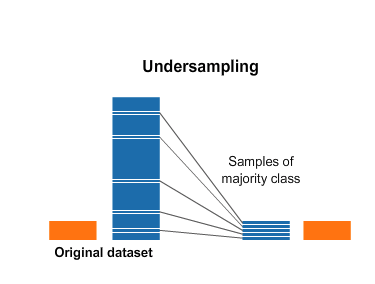
\includegraphics[width=.7\textwidth]{figures/Undersampling.png}
\caption{Undersampling Technique \cite{OverUnderIbm2019}}
\label{fig:undersampling}
\end{figure}

It involves removing samples from the dataset until the data
is balanced. The reasons to use under-sampling are usually related to practical 
reasons, such as resource costs. The techniques presented are:

\paragraph{Random Undersampling}

It involves deleting samples from the majority class, with or without 
replacement.It is one of the early proposals to deal with imbalanced datasets.
Although it may alleviate the imbalance in the dataset, it may also increase the
variance of the classifier or discard meaningful samples from the majority 
class.

\paragraph{Cluster Centroid}

It replaces a cluster of samples by the cluster centroid of a K-means 
algorithm. The number of clusters is set by the level of undersampling.

\paragraph{Near Miss}\label{nearmiss}

Refers to a collection of undersampling methods that select samples based on 
the distance of the majority class samples to the minority class 
samples~\cite{Zhang03}. There are three versions of this algorithm: 
(1) \textit{NearMiss-1} selects majority class samples with minimum average
distance to three closest minority class samples; 
(2) \textit{NearMiss-2} selects majority class examples with minimum average 
distance to the three furthest minority class examples;
(3) \textit{NearMiss-3} selects majority class examples with minimum distance 
to each minority class example.

Among all the available techniques, \textit{Near Miss} has been the on used
for this research.

Other techniques that remove instances intelligently include the Edited Nearest
Neighbor (ENN) and Wilson's Editing that remove instances in which close 
neighbors belong to a  different class~\cite{wilson1972asymptotic}.

%%%%%%%%%%%%%%%%%%%%%%%%%%%%%%%%%%%%%%%%%%%%%%%%%%%%%%%%%%%%
\subsubsection{Oversampling}

\begin{figure}[h!]
\centering
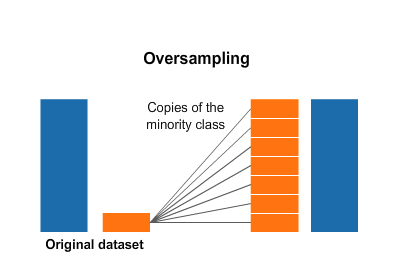
\includegraphics[width=.7\textwidth]{figures/Oversampling.png}
\caption{Oversampling Technique \cite{OverUnderIbm2019}}
\label{fig:oversampling}
\end{figure}

Most commonly used. It involves creating new data points from the already 
existing data. The techniques analyzed are:

\paragraph{Random Oversampling}. Involves copying supplementary data from the
minority classes. It can be done more than once (actually, as many times as the
developers sees fit). One of the early proposals regarding imbalanced datasets.
It is robust, as it may randomly replace some of the samples from the minority 
class.

\paragraph{SMOTE}\label{smote}

Acronym for Synthetic Minority Oversampling Technique~\cite{ChawlaBHK02}. 
It is one of the most popular techniques used nowadays. It works by selecting 
samples close in the feature space. That means, that a line is drawn between
the samples in the feature space and the a new sample at a point along that 
line. It is effective because the samples from the minority class created are
plausible - relatively close in feature space to existing samples from minority 
class. A downside of this technique is that samples are created without looking
at the majority class, meaning a possible overlapping of classes.

\paragraph{ADASYN}

Acronym for ADaptative SYNthetic sampling algorithm. Build on SMOTE methodology.
Shifts the importance of the classification boundary to those minority classes 
which are difficult. Weights the most difficult to learn classes so that those
have more importance when creating new data. ADASYN generates more synthetic 
data in the minority class samples that are harder to learn.

The technique selected for this article is the SMOTE method, implemented by the 
\textit{imblearn} Python package.

%%%%%%%%%%%%%%%%%%%%%%%%%%%%%%%%%%%%%%%%%%%%%%%%%%%%%%%%%%%%%%%%%%%
\subsection{Cost-Sensitive Classifiers}\label{subsec:costSensitive}

Also known as CSC. These are adapted classifiers that handle imbalanced 
datasets by either:

\begin{enumerate}
    \item Adding weights to instances\footnote{Can only be used if the base 
    classifier algorithm allows it}.
    \item Resampling the training data according to the costs assigned to each 
    class in a predefined cost matrix.
    \item Or generating a model that minimizes the expected cost\footnote{Can 
    be obtained by multiplying the predicted probability distribution with the 
    misclassification costs}. The idea behind this methodology is to penalize 
    differently each type of error - in the specific case of binary 
    classification, the false positives (FP) and false negatives (FN).
\end{enumerate}

The problem with CSC is defining the cost matrix as there is no systematic 
approach to do so. However, it is common practice to set the cost to equalize 
the class distribution.

%%%%%%%%%%%%%%%%%%%%%%%%%%%%%%%%%%%%%%%%%%%%%%%%%%%%%%%%%%%%%%%%%%%
\subsection{Ensembles}\label{sec:ensembles}

Also known as meta-learners are a combination of multiple models with the 
objective of obtaining better predictions. They are typically classified as 
\emph{Bagging}, \emph{Boosting} and \emph{\emph{Stacking}} - Stacked 
generalization.

%%%%%%%%%%%%%%%%%%%%%%%%%%%%%%%%%%%%%%%%%%%%%%%%%%%%%%%%%%%%
\subsubsection{Bagging}

Bagging~\cite{Breiman96} (also known as Bootstrap aggregating) is a ensemble 
technique that involves a base learner applied to multiple - equal size - 
datasets. These datasets are created from the original data using bootstraping. 
Predictions are made on voting of the individual predictions. 

An advantage of this technique is that it does not require to modify
any aspect of the learning algorithm, taking advantage of the instability of 
the base classifier to create diversity among individual ensembles - so that 
individual members of the ensemble perform well in different regions of the 
data.  

If the output is robust to perturbation of the data (like is the case with
nearest-neighbor (NN) classifiers) the performance drops.

%%%%%%%%%%%%%%%%%%%%%%%%%%%%%%%%%%%%%%%%%%%%%%%%%%%%%%%%%%%%
\subsubsection{Boosting}

Boosting techniques generate multiple models that complement each other. The
final objective is to induce models that improve certain regions of the data,
where previous induced models had low performance. This can be achieved by 
increasing the weights of instances that have been wrongly classified. That 
way, new learners focus on those regions. 

Classification is based on a weighted voted among all members of the ensemble.
One of the most popular boosting algorithms is AdaBoost.M1~\cite{Freund1996} 
for classification. The set of training examples is assigned an equal weight 
at the beginning and the weight of instances can be increased or decreased 
depending on the classification of the learner. The next iterations focus on 
those instances with higher weights. AdaBoost.M1 can be applied to any base 
learner.

Models from ensembles are difficult to interpret (black box behavior), 
comparing them to decision trees or rules providing explanation of their 
decision making process.

%%%%%%%%%%%%%%%%%%%%%%%%%%%%%%%%%%%%%%%%%%%%%%%%%%%%%%%%%%%%%%%%%%%%%%
\subsection{Hybrid Approaches}\label{subsec:hybridApproaches}

There are other hybrid approaches that can be used. Like that ones that
are going to be explained in the following section.

%%%%%%%%%%%%%%%%%%%%%%%%%%%%%%%%%%%%%%%%%%%%%%%%%%%%%%%%%%%%
\subsubsection{SMOTEBoost}

The SMOTEBoost tries to reduce the bias from the learning procedure due to 
the class imbalance, and increase the sampling weight for the minority class. 
SMOTE~\cite{CBHK2002} is introduced in each round of boosting, which enables
each learner to be able to sample more of the minority class cases, and
learn better and broader decision regions for the minority class. 

It also brings the benefit of enhancing the probability of selection for 
the difficult minority class cases that are dominated by the majority class 
points~\cite{CLHB2003}. The variation of boosting procedure of the SMOTEBoost
process is a variant of the AdaBoost.M2 procedure~\cite{FS1997}.

%%%%%%%%%%%%%%%%%%%%%%%%%%%%%%%%%%%%%%%%%%%%%%%%%%%%%%%%%%%%
\subsubsection{RUSBoost}

The technique RUSBoost~\cite{Seiffert2010} uses the AdaBoost.M2. The 
difference with SMOTEBoost is that RUSBoost applies Random Under Sampling 
instead of SMOTE. The application of SMOTE at this point has two drawbacks that 
RUSBoost is designed to overcome:

\begin{itemize}
    \item Increases the complexity of the algorithm. SMOTE finds the $k$ 
    nearest neighbors of the minority class samples, and then extrapolates
    them to make new synthetic samples. RUS, on the other hand, simply deletes 
    the majority class examples randomly.
    \item RUS produces less training datasets (as it is an undersampling 
    technique, not like SMOTE, which is an oversampling technique). This can
    be translated into shorter model training times~\cite{Seiffert2010}.
\end{itemize}

%%%%%%%%%%%%%%%%%%%%%%%%%%%%%%%%%%%%%%%%%%%%%%%%%%%%%%%%%%%%
\subsubsection{MetaCost}

MetaCost~\cite{Domingos1999} is a combination of bagging with cost-sensitive 
classification. The bagging part of the technique is used to relabel training 
data so that each training example is assigned a prediction that minimizes the 
expected cost for that instance. Based on the modified training data, MetaCost 
induces a new classifier which provides information about how a decision was 
reached.

%%%%%%%%%%%%%%%%%%%%%%%%%%%%%%%%%%%%%%%%%%%%%%%%%%%%%%%%%%%%%%%%%%%%%%
\subsection{Defect Prediction}\label{subsec:defectPrediction}

Regarding the history of defect prediction, and final objective of this 
article, many classification techniques have been proposed - statistics
(regression~\cite{Bibi06}, and Support Vector Machines~\cite{Elish2008}, etc.),
machine learning (classification trees~\cite{Khoshgoftaar02}), neural 
networks~\cite{Khoshgoftaar97}), probability (Na\"ive Bayes~\cite{Menzies07b} 
and Bayesian networks), ensembles of different techniques and meta-heuristics
(ant colonies~\cite{Vandecruys2008}, etc.).

Despite this fact, some discrepancies are found:

\begin{itemize}
    \item No classifier is consistently better than others.
    \item There is no optimum metric that allows the evaluation and comparison
    of classifiers (\cite{Mende09,Zhang07,Menzies07b}).
    \item Data is also affected by quality issues - class imbalance, 
    overlapping, outliers, etc.).
\end{itemize}

Some authors highlight the problem of imbalanced datasets when dealing with
the project at hand, defect prediction (Seiffert et al.~\cite{Seiffert2009} and 
in Khoshgoftaar et al.~\cite{Khoshgoftaar03}).

As it has been mentioned before, there is no classifier that behaves 
consistently better. No technique is able to give a an outstanding performance 
when evaluating classifiers. Some authors have compared performance of several
measures (like Peng~\cite{Peng2009}, Peng et al.~\cite{Peng2010}, this papers
actually propose performance metrics to evaluate merit of classification 
algorithms and ranked classification algorithms, respectively).

Further made on the subject comes from the hand of Lessman et al.~\cite{LBMP08}.
This paper compared several classifiers, discussing performance metrics such 
like $TP_r$ and $FP_r$. But finally advocated to use the AUC\footnote{Further 
explained in Section~\ref{sec:roc}, Area Under the ROC curve} as the best 
indicator for classifiers comparison. This results is known as sub-optimal for 
highly imbalanced datasets.

Arisholm et al.~\cite{Arisholm10} compared different classification
algorithms (tree algorithm (C4.5), coverage rule algorithm (PART), logistic 
regression, back-propagation neural networks and Support Vector Machines) over 
13 different Java developed systems. They used three metrics to compare results:

\begin{itemize}
    \item Object-oriented metrics.
    \item Churn ($\delta$) metrics between successive releases.
    \item Process management metrics from a configuration management system.
\end{itemize}

The conclusion was that large differences can be achieved depending on the 
comparison criteria of the data. To solve this problem, the paper proposed
a new AUC based, cost-effectiveness metric. Same approach has been evaluated 
and explored in Mende and Koschke~\cite{Mende10}.
